\documentclass[12pt]{article}


\usepackage{mystyle}
\setmonofont{SF Mono}
\graphicspath{{src/}}

\pagestyle{fancy}
\fancyhf{}
\rhead{High Frequency Communication Systems}
\lhead{Lab Manual 1 - FDTD}
\rfoot{\thepage}
\begin{document}

In this lab session, you will learn about:
\begin{outline}
  \1 2D FDTD
  \1 Stability Conditions
  \1 Boundary Conditions
\end{outline}

As discussed in the class, we are only going to compute only one field component at a time. Moreover, the corner points are not considered when it comes to computing the fields. This is because of the \textit{wedge condition} due to which the fields shoot to infinity. The last observation is that we need to space the computation parts uniformly across the whole region of space.

In this lab session, we look at the higher dimension cases of FDTD a bit closely. We will be using some \texttt{MATLAB} routines for this purpose. One marked difference is that we are going to define the update coefficients so that material properties can be introduced more efficiently.

Using the discretisation approach that we learnt in the class, we can represent any point in space that is transformed from a continuous domain to a discrete domain $(i\Delta x,j\Delta y,k \Delta z)$.

After doing this, we can then express any function $u$ in the finite difference notation in terms of space and time as:
\begin{align}
  u(i\Delta x,j\Delta y,k \Delta z, n \Delta t) & = u_{i,j,k}^n
\end{align}

As shown in Fig. \ref{fig:yee_lattice}, we can programatically express the space coordinates $x$,$y$, and $z$ with the variable $i$, $j$, and $k$ respectively. For time $t$ , the variable $n$ is reserved.

\begin{figure}[h!]
  \centering
  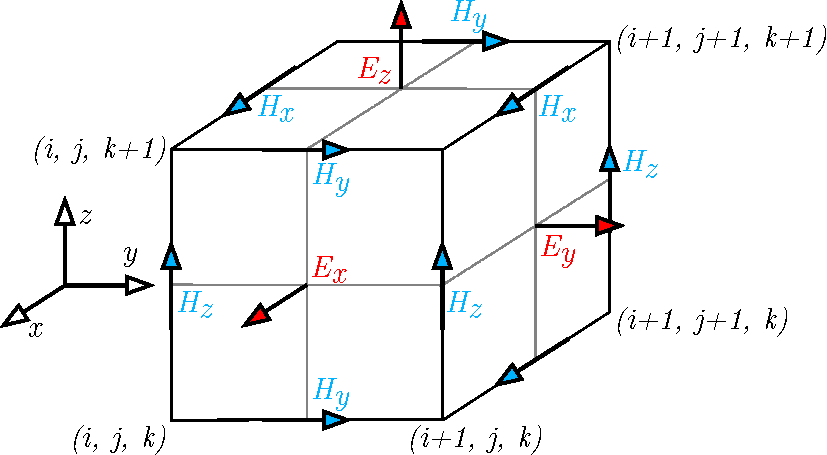
\includegraphics[width=.5\textwidth]{yee lattice.pdf}
  \caption{The Yee Lattice showing the space indices and field computation points.}
  \label{fig:yee_lattice}
\end{figure}

The spacing chosen by Yee in his algorithm produces a $1/2$ increment calculation in space:

\begin{align}
  \pdv{u (i \Delta x, j \Delta y, k \Delta z, n \Delta y )}{x} & = \frac{u^n_{i + 1/2, j , k} - u^n_{i - 1/2, j , k}}{\Delta x} + \mathcal{O}\left[(\Delta x)^2\right]
\end{align}

Similarly, the time derivative was also chosen to be at $1/2$ time increments:

\begin{align}
  \pdv{u (i \Delta x, j \Delta y, k \Delta z, n \Delta y )}{t} & = \frac{u^{n + 1/2}_{i , j , k} - u^{n - 1/2}_{i , j , k}}{\Delta t} + \mathcal{O}\left[(\Delta t)^2\right]
\end{align}

\section{Finite Difference Time-Domain method}

For the sake of complying with duality we introduced a magnetic current term in the Maxwell's equations. Although, there is no physical basis for it, yet the term is introduced so that dual of the electric current is present in the Ampere's law:

\begin{subequations}
  \begin{align}
    \pdv{\va{E}}{t} & = \frac{1}{\E} \curl{\va{H}} - \frac{\sigma}{\E}  \va{E} \label{eq:faradays}   \\
    \pdv{\va{H}}{t} & = -\frac{1}{\u} \curl{\va{E}} - - \frac{\rho'}{\u}  \va{H} \label{eq:ameperes}
  \end{align}
  \label{eq:maxwell}
\end{subequations}

where the terms $\rho'$, and $\sigma$ refer to the magnetic resistivity and electrical conductivity. In three dimensions, the magnetic fields from \eqref{eq:maxwell} can be written as:

\begin{subequations}
  \begin{align}
    \pdv{H_x}{t} & =\frac{1}{\u}\left(\pdv{E_y}{z}-\pdv{E_z}{y}-\rho' H_{x}\right) \label{eq:H_x_3D} \\
    \pdv{H_y}{t} & =\frac{1}{\u}\left(\pdv{E_z}{x}-\pdv{E_x}{z}-\rho' H_{y}\right) \label{eq:H_y_3D} \\
    \pdv{H_z}{t} & =\frac{1}{\u}\left(\pdv{E_x}{y}-\pdv{E_y}{x}-\rho' H_{z}\right) \label{eq:H_z_3D}
  \end{align}
  \label{eq:magnetic}
\end{subequations}

and the electric fields as:

\begin{subequations}
  \begin{align}
    \pdv{E_x}{t} & =\frac{1}{\E}\left(\pdv{H_z}{y}-\pdv{H_y}{z}-\sigma E_{x}\right) \label{eq:E_x_3D} \\
    \pdv{E_y}{t} & =\frac{1}{\E}\left(\pdv{H_x}{z}-\pdv{H_z}{x}-\sigma E_{y}\right) \label{eq:E_y_3D} \\
    \pdv{E_z}{t} & =\frac{1}{\E}\left(\pdv{H_y}{x}-\pdv{H_x}{y}-\sigma E_{z}\right) \label{eq:E_z_3D}
  \end{align}
  \label{eq:electric}
\end{subequations}

As an example, the central difference approximation for \eqref{eq:H_x_3D} becomes:

\begin{align}
  \frac{\left. H_{x} \right|^{n + 1/2}_{i,j,k} - \left. H_{x} \right|^{n - 1/2}_{i,j,k}}{\Delta t}  = \frac{1}{\u_{i,j,k}}
  \left[
  \frac{\left. E_y \right|^{n}_{i,j,k+1/2} - \left. E_y \right|^{n}_{i,j,k-1/2}}{\Delta z}  \right. \nonumber \\
  \left. - \frac{\left. E_z \right|^{n}_{i,j+1/2,k} - \left. E_y \right|^{n}_{i,j-1/2,k}}{\Delta y} - \rho'_{i,j,k} \left. H_x \right|^{n}_{i,j,k}
  \right]                                                        \label{eq:H_x_3d_central_difference}
\end{align}

Notice that in \eqref{eq:H_x_3d_central_difference}, $\va{E}$ and $\va{H}$ exist $1/2$ time step apart. As the electric fields occupy the time step $n$, the magnetic fields only exist at half-time step $n - 1/2$, or  $n + 1/2$. This means that $\left. H_x \right|^n_{i,j,k}$ needs to be \textit{approximated}. Often times, we just use the average:

\begin{align}
  \left. H_x \right|^n_{i,j,k} & = \frac{\left. H_x \right|^{n+1/2}_{i,j,k} + \left. H_x \right|^{n-1/2}_{i,j,k}}{2}
  \label{eq:H_averaged}
\end{align}

From \eqref{eq:H_x_3d_central_difference} and \eqref{eq:H_averaged} we get:

\begin{align}
  \left. H_{x} \right|^{n + 1/2}_{i,j,k} - \left. H_{x} \right|^{n - 1/2}_{i,j,k} = \frac{\Delta t}{\u_{i,j,k}}
  \left[
  \frac{\left. E_y \right|^{n}_{i,j,k+1/2} - \left. E_y \right|^{n}_{i,j,k-1/2}}{\Delta z} - \right. \nonumber \\
  \left. \frac{\left. E_z \right|^{n}_{i,j+1/2,k} - \left. E_y \right|^{n}_{i,j-1/2,k}}{\Delta y}
  \right]
  \label{eq:solving_H_3d}
\end{align}

After collecting $\left. H_{x} \right|^{n + 1/2}_{i,j,k}$ and $\left. H_{x} \right|^{n - 1/2}_{i,j,k}$, we get:

\begin{align}
  \left( 1 + \frac{\Delta t}{\u_{i,j,k}} \frac{\rho'_{i,j,k}}{2}\right) \left. H_{x} \right|^{n + 1/2}_{i,j,k} = \left( 1- \frac{\Delta t}{\u_{i,j,k}}\frac{\rho'_{i,j,k}}{2}\right) \left. H_{x} \right|^{n - 1/2}_{i,j,k}   \nonumber \\
  +  \frac{\Delta t}{\u_{i,j,k}} \left[
  \frac{\left. E_y \right|^{n}_{i,j,k+1/2} - \left. E_y \right|^{n}_{i,j,k-1/2}}{\Delta z} - \frac{\left. E_z \right|^{n}_{i,j+1/2,k} - \left. E_y \right|^{n}_{i,j-1/2,k}}{\Delta y}
  \right]
  \label{eq:further_simplifying_H_y_3D}
\end{align}


Dividing \eqref{eq:further_simplifying_H_x_3D} by dividing by $\left( 1 + \frac{\Delta t}{\u_{i,j,k}} \frac{\rho'_{i,j,k}}{2}\right)$, we get:

\begin{align}
  \left. H_{x} \right|^{n + 1/2}_{i,j,k} ={} & \underbrace{\left(
    \frac{1 - \frac{\rho'_{i,j,k} \Delta t}{2 \u_{i,j,k}}}{1 + \frac{\rho'_{i,j,k} \Delta t}{2 \u_{i,j,k}}}
  \right)}_{D_{a,\left. H_{x} \right|_{i,j,k}}} \left. H_{x} \right|^{n - 1/2}_{i,j,k} \nonumber                                                                                                                                                  \\
                                              & + \underbrace{\left(
    \frac{\frac{\Delta t}{\u_{i,j,k}}}{1 + \frac{\rho'_{i,j,k} \Delta t}{2 \u_{i,j,k}}}
    \right)}_{D_{b,\left. H_{x} \right|_{i,j,k}}} \left[
  \frac{\left. E_y \right|^{n}_{i,j,k+1/2} - \left. E_y \right|^{n}_{i,j,k-1/2}}{\Delta z} - \right. \nonumber                                                                                                                                    \\
                                              & \left. \frac{\left. E_z \right|^{n}_{i,j+1/2,k} - \left. E_y \right|^{n}_{i,j-1/2,k}}{\Delta y} - \rho'_{i,j,k} \frac{\left. H_x \right|^{n+1/2}_{i,j,k} + \left. H_x \right|^{n-1/2}_{i,j,k}}{2}
  \right]
  \label{eq:final_Hx_3D}
\end{align}

Using the same procedures, we can find out the expressions for other components of the magnetic field:


\begin{subequations}
  \begin{align}
    \left. H_{y} \right|^{n + 1/2}_{i,j,k} ={} & \underbrace{\left(
      \frac{1 - \frac{\rho'_{i,j,k} \Delta t}{2 \u_{i,j,k}}}{1 + \frac{\rho'_{i,j,k} \Delta t}{2 \u_{i,j,k}}}
    \right)}_{D_{a,\left. H_{y} \right|_{i,j,k}}} \left. H_{y} \right|^{n - 1/2}_{i,j,k}  \nonumber                                                  \\
                                                & + \underbrace{\left(
      \frac{\frac{\Delta t}{\u_{i,j,k}}}{1 + \frac{\rho'_{i,j,k} \Delta t}{2 \u_{i,j,k}}}
      \right)}_{D_{b,\left. H_{y} \right|_{i,j,k}}} \left[
    \frac{\left. E_z \right|^{n}_{i+1/2,j,k} - \left. E_z \right|^{n}_{i-1/2,j,k}}{\Delta x}  \right. \nonumber                                      \\
                                                & \left. - \frac{\left. E_x \right|^{n}_{i,j,k+1/2} - \left. E_x \right|^{n}_{i,j,k-1/2}}{\Delta z}
    \right] \label{eq:final_Hy_3D}                                                                                                                     \\
    \left. H_{z} \right|^{n + 1/2}_{i,j,k} c  \underbrace{\left(
      \frac{1 - \frac{\rho'_{i,j,k} \Delta t}{2 \u_{i,j,k}}}{1 + \frac{\rho'_{i,j,k} \Delta t}{2 \u_{i,j,k}}}
    \right)}_{D_{a,\left. H_{z} \right|_{i,j,k}}} \left. H_{z} \right|^{n - 1/2}_{i,j,k} + \nonumber                                                 \\
                                                & \underbrace{\left(
      \frac{\frac{\Delta t}{\u_{i,j,k}}}{1 + \frac{\rho'_{i,j,k} \Delta t}{2 \u_{i,j,k}}}
      \right)}_{D_{b,\left. H_{z} \right|_{i,j,k}}} \left[
    \frac{\left. E_x \right|^{n}_{i,j+1/2,k} - \left. E_x \right|^{n}_{i,j-1/2,k}}{\Delta y}  \right. \nonumber                                     \\
                                                & \left. -  \frac{\left. E_y \right|^{n}_{i+1/2,j,k} - \left. E_y \right|^{n}_{i-1/2,j,k}}{\Delta x}
    \right] \label{eq:final_Hz_3D}
  \end{align}
\end{subequations}

Similarly, the electric field components are:

\begin{subequations}
  \begin{align}
    \left. E_{x} \right|^{n + 1}_{i,j,k} ={} & \underbrace{\left(
      \frac{1 - \frac{\sigma_{i,j,k} \Delta t}{2 \E_{i,j,k}}}{1 + \frac{\sigma_{i,j,k} \Delta t}{2 \E_{i,j,k}}}
    \right)}_{C_{a,\left. E_{x} \right|_{i,j,k}}} \left. E_{x} \right|^{n}_{i,j,k} \nonumber                                                              \\
                                              & + \underbrace{\left(
      \frac{\frac{\Delta t}{\E_{i,j,k}}}{1 + \frac{\sigma_{i,j,k} \Delta t}{2 \E_{i,j,k}}}
      \right)}_{C_{b,\left. E_{x} \right|_{i,j,k}}} \left[
    \frac{\left. H_z \right|^{n+1/2}_{i,j+1/2,k} - \left. H_z \right|^{n+1/2}_{i,j-1/2,k}}{\Delta y}  \right. \nonumber                                   \\
                                              & \left. - \frac{\left. H_y \right|^{n+1/2}_{i,j,k+1/2} - \left. H_y \right|^{n+1/2}_{i,j,k-1/2}}{\Delta z}
    \right] \label{eq:final_Ex_3D}                                                                                                                          \\
    \left. E_{y} \right|^{n + 1}_{i,j,k} ={} & \underbrace{\left(
      \frac{1 - \frac{\sigma_{i,j,k} \Delta t}{2 \E_{i,j,k}}}{1 + \frac{\sigma_{i,j,k} \Delta t}{2 \E_{i,j,k}}}
    \right)}_{C_{a,\left. E_{y} \right|_{i,j,k}}} \left. E_{y} \right|^{n}_{i,j,k} \nonumber                                                              \\
                                              & + \underbrace{\left(
      \frac{\frac{\Delta t}{\E_{i,j,k}}}{1 + \frac{\sigma_{i,j,k} \Delta t}{2 \E_{i,j,k}}}
      \right)}_{C_{b,\left. E_{y} \right|_{i,j,k}}} \left[
    \frac{\left. H_x \right|^{n+1/2}_{i,j,k+1/2} - \left. H_x \right|^{n+1/2}_{i,j,k-1/2}}{\Delta z}  \right. \nonumber                                   \\
                                              & \left. - \frac{\left. H_z \right|^{n+1/2}_{i+1/2,j,k} - \left. H_z \right|^{n+1/2}_{i-1/2,j,k}}{\Delta x}
    \right] \label{eq:final_Ey_3D}                                                                                                                          \\
    \left. E_{z} \right|^{n + 1}_{i,j,k} ={} & \underbrace{\left(
      \frac{1 - \frac{\sigma_{i,j,k} \Delta t}{2 \E_{i,j,k}}}{1 + \frac{\sigma_{i,j,k} \Delta t}{2 \E_{i,j,k}}}
    \right)}_{C_{a,\left. E_{z} \right|_{i,j,k}}} \left. E_{z} \right|^{n}_{i,j,k} \nonumber                                                              \\
                                              & + \underbrace{\left(
      \frac{\frac{\Delta t}{\E_{i,j,k}}}{1 + \frac{\sigma_{i,j,k} \Delta t}{2 \E_{i,j,k}}}
      \right)}_{C_{b,\left. E_{z} \right|_{i,j,k}}} \left[
    \frac{\left. H_y \right|^{n+1/2}_{i+1/2,j,k} - \left. H_y \right|^{n+1/2}_{i-1/2,j,k}}{\Delta x} \right. \nonumber                                    \\
                                              & \left. - \frac{\left. H_x \right|^{n+1/2}_{i,j+1/2,k} - \left. H_x \right|^{n+1/2}_{i,j-1/2,k}}{\Delta y}
    \right] \label{eq:final_Ez_3D}
  \end{align}
\end{subequations}

Our goal will be to define the update coefficients $C$ and $D$ when we need to create inhomogeneous medium simulations. As an example, when the conductivity $\sigma$ and magnetic resistivity $\rho'$ are both equal to zero, the coefficients become,

\begin{subequations}
  \begin{align}
    D_{a,\left. H_{x,y,z} \right|_{i,j,k}} ={} & 1                           \\
    D_{b,\left. H_{x,y,z} \right|_{i,j,k}} ={} & \frac{\Delta t}{\u_{i,j,k}} \\
    C_{a,\left. E_{x,y,z} \right|_{i,j,k}} ={} & 1                           \\
    C_{b,\left. E_{x,y,z} \right|_{i,j,k}} ={} & \frac{\Delta t}{\E_{i,j,k}} \\
  \end{align}
  \label{eq:coefficients}
\end{subequations}

For the $2D$ case we assume $(\pdv{z} = 0)$, and then write the uncoupled expressions as $TM$ and $TE$ modes:

\textit{TM mode}:

\begin{subequations}
  \begin{align}
    \pdv{H_x}{t} ={} & \frac{1}{\u}\left(-\pdv{E_z}{y}-\rho' H_{x}\right)     \label{eq:H_x_TM}          \\
    \pdv{H_y}{t} ={} & \frac{1}{\u}\left(\pdv{E_z}{x}-\rho' H_{y}\right)    \label{eq:H_y_TM}            \\
    \pdv{E_z}{t} ={} & \frac{1}{\E}\left(\pdv{H_y}{x}-\pdv{H_x}{y}-\sigma E_{z}\right) \label{eq:E_z_TM}
  \end{align}
  \label{eq:TM mode}
\end{subequations}

\textit{TE mode}:

\begin{subequations}
  \begin{align}
    \pdv{E_x}{t} ={} & \frac{1}{\E}\left(\pdv{H_z}{y}-\sigma E_{x}\right)      \label{eq:E_x_TE}        \\
    \pdv{E_y}{t} ={} & \frac{1}{\E}\left(-\pdv{H_z}{x}-\sigma E_{y}\right)    \label{eq:E_y_TE}         \\
    \pdv{H_z}{t} ={} & \frac{1}{\u}\left(\pdv{E_x}{y}-\pdv{E_y}{x}-\rho' H_{z}\right) \label{eq:H_z_TE}
  \end{align}
  \label{eq:TE mode}
\end{subequations}

Using the coefficients in \eqref{eq:coefficients}, the 2D $TM$ mode central difference equations from \eqref{eq:TM mode} are:
\begin{subequations}
  \begin{align}
    \left. H_{x} \right|^{n + 1/2}_{i,j} ={} & \left. H_x \right|^{n - 1/2}_{i,j} - \frac{\Delta t}{\u_{i,j}} \left[\frac{\left. E_z \right|^{n }_{i,j+1/2} - \left. E_z \right|^{n}_{i,j-1/k2}}{\Delta y}\right]                                                        \label{eq:H_x_TM_central_difference}      \\
    \left. H_{y} \right|^{n + 1/2}_{i,j} ={} & \left. H_y \right|^{n - 1/2}_{i,j} - \frac{\Delta t}{\u_{i,j}} \left[\frac{\left. E_z \right|^{n }_{i+1/2,j} - \left. E_z \right|^{n}_{i-1/2,j}}{\Delta x}\right]                                                          \label{eq:H_y_TM_central_difference}     \\
    \left. E_{z} \right|^{n + 1}_{i,j}   ={} & \left. E_z \right|^{n}_{i,j} - \frac{\Delta t}{\E_{i,j}} \left[\frac{\left. H_y \right|^{n+1/2}_{i+1/2,j} - \left. H_y \right|^{n+1/2}_{i-1/2,j}}{\Delta x} - \frac{\left. H_x \right|^{n+1/2}_{i,j+1/2} - \left. H_x \right|^{n+1/2}_{i,j-1/2}}{\Delta y}\right]
    \label{eq:E_z_TM_central_difference}
  \end{align}
  \label{eq:update_eqs_TM}
\end{subequations}

\section{Programming the equations}

We look to solve the 2D TM mode case; the rest of the cases follow a similar approach.

\begin{outline}[enumerate]
  \1 Before we perform the time-stepping of the fields, we compute all the update coefficients $C_{a,b}$ and $D_{a,b}$ and store them in an array. These will remain unchanged.
  \1 We compute the magnetic fields \textcolor{red}{2 time-steps} back, ie. $\left. H_x \right|^{n - 1/2}_{i,j}$ and $\left. H_y \right|^{n - 1/2}_{i,j}$ and store them in the array \texttt{Hx(i,j)} and \texttt{Hy(i,j)} respectively.
  \1 We then compute the electric field \texttt{Ez(i,j)} \textcolor{red}{1 time-step} back ($\left. E_z \right|^{n}_{i,j}$).
  \1 At the current time, which is always $n + 1/2$, the magnetic field components, $\left. H_x \right|^{n + 1/2}_{i,j}$ and $\left. H_y \right|^{n + 1/2}_{i,j}$ are computed and the magnetic field array is updated accordingly.
  \1 In the next time step, $\left. E_z \right|^{n+1}_{i,j}$ is computed and stored in the \texttt{Ez(i,j)} array where we replace the value $\left. E_z \right|^{n}_{i,j}$ with the new one.
  \1 As the updating of the $E$ and $H$ actually implements the time-stepping, we need to have a time index explicitly.
\end{outline}

Now let's look at a \texttt{Matlab} routine that implements the 2D TM mode fields in a rectangular space with perfect electric (PEC) boundaries.

\begin{mdframed}[backgroundcolor=gray!20]
  \scriptsize
  \begin{minted}{matlab}
% This program computes and plots the TM mode fields in 
% 2D rectagnular space with PEC boundaries using 
% Yee's FDTD Algorithm. 
%
%% Define Parameters
c = 2.99792458e8; % Speed of light
eps0 = 8.854187817e-12; % Free space permittivity
xmu0 = 4*pi*1e-7; % Free space permeability
%
%%  Define Space Region
a = 10; b = 10; % Space Dimensions
% Number of grid points in x and y direction
nx = 100; ny = 100; 
% Convert to integer in-case of odd number
nx2 = ceil(nx/2); ny2 = ceil(ny/2); 
nt = 200; % Number of time-steps
nskip = 5; % Time-steps to skip while recording
nsnap = ceil(nt/nskip);
%
%% Create a Gaussian Excitation Source
xndec = 10.0; % Mean
xn0 = 4*xndec; % Variance
%
%% Initialize
%
Ez = zeros( nx, ny ); %  Z E-field initialize to zero
Hx = zeros( nx, ny ); %  X H-field initialize to zero
Hy = zeros( nx, ny ); %  Y H-field initialize to zero

dx = a/(nx - 1); % Define spatial step
dy = dx; %
ds = dx;

% **************************
% **************************
dt = ds/(c*sqrt(2)); % Stability Condition
% **************************
% **************************

\end{minted}
\end{mdframed}

The approach of the Yee algorithm along with the material definition follows what has been described in \cite[pg. 85]{taflove_computational_2005}. The medium is defined as:

\begin{mdframed}[backgroundcolor=gray!20]
  \scriptsize
  \begin{minted}{matlab}
%% Medium Definition
%
dte = ones(nx,ny)*dt/(ds*eps0);
dtm = ones(nx,ny)*dt/(ds*xmu0);
Da = ones(nx,ny);
Db = dtm;
Ca = ones(nx,ny);
Cb = dte;
%
  \end{minted}
\end{mdframed}

Next, we implement the Yee algorithm:

\begin{mdframed}[backgroundcolor=gray!20]
  \scriptsize
  \begin{minted}{matlab}
%% Yee Algorithm
for n = 1:nt
    for i = 1 : nx
        for j = 1 : ny
            if (i == nx2 && j == ny2) % Place source in the center
                
                Ez(i,j) = exp(-((n-xn0)/(xndec))^2); % Gaussian Source
                
            elseif (i == 1 || j == 1 || i == nx || j == ny )
                
                Ez(i,j) = 0; % PEC boundaries at the edges
                
            else
                
                Ez(i,j) = Ez(i,j)*Ca(i,j) + Cb(i,j)*(Hy(i,j) - Hy(i-1,j)...
                    - (Hx(i,j) - Hx(i,j-1)));
                
            end
        end
    end
    
    for i = 1 : nx
        for j = 1 : ny - 1
            
            Hx(i,j) = Hx(i,j)*Da(i,j) - Db(i,j)*(Ez(i,j+1) - Ez(i,j));
            
        end
    end
    
    for i = 1 : nx - 1
        for j = 1 : ny
            
            Hy(i,j) = Hy(i,j)*Da(i,j) + Db(i,j)*(Ez(i+1,j) - Ez(i,j));
            
        end
    end
end
  \end{minted}
\end{mdframed}

\normalsize
We can use the plotting routine below to visualise the electric fields:
\begin{mdframed}[backgroundcolor=gray!20]
  \scriptsize
  \begin{minted}{matlab}
    %% Plot Routine
%
xd = 0:ds:a;
[xdg, ydg] = meshgrid(xd, xd);
figure(1)
EzSurf = surf(xdg,ydg,Ez,'EdgeColor','interp','FaceLighting','gouraud');
shading interp % Avoid jittered shading
set(gcf,'Color','white'); % Set background color to white
set (gca,'FontName','times new roman') % Set axes fonts to Times New Roman
box on %
colorbar % Show colorbar on the right of the figure
grid on
colormap('jet')
material dull % Set reflectivity of the surface to dull
% Add three lights below tom improve visuals
h = light;
light('Position',[10 0 1]);
light('Position',[-190 -120 1]);
light('Position',[0 0 1]);
title(['E-field at Time Step ',int2str(n)])
% Create Title with mode numbers
matFileName = sprintf('E_Field_%d', n);

if rem(n,nskip) == 0
    
    M_PEC(:,n/nskip) = getframe; % Capture frames to create a movie
    
end

if n == 20 || n == 60 || n == 80 || n == 100 ||...
        n == 120 || n == 140 || n == 160
    saveas(gcf,[matFileName,'.eps'],'epsc') % Save visualizations
end
  \end{minted}
\end{mdframed}

Running the Matlab file, we should get a 2D Gaussian source starting from the origin and expanding outwards as seen in the figure below:

\begin{figure}[!htbp]
  \centering
  \subfloat[20]{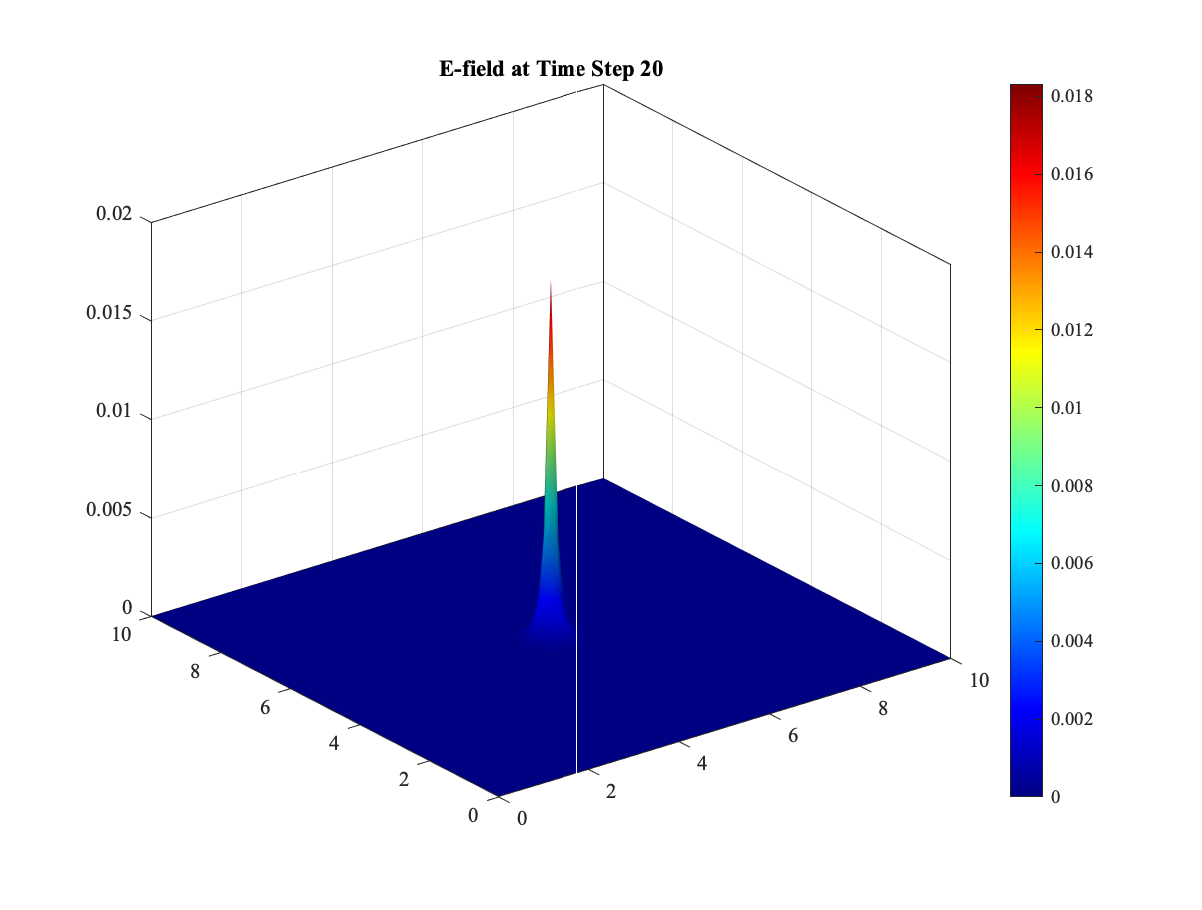
\includegraphics[width=2.5in]{Abbas_3_7_E_Field_20.eps}
  \label{fig:field_at_20}}
  \subfloat[60]{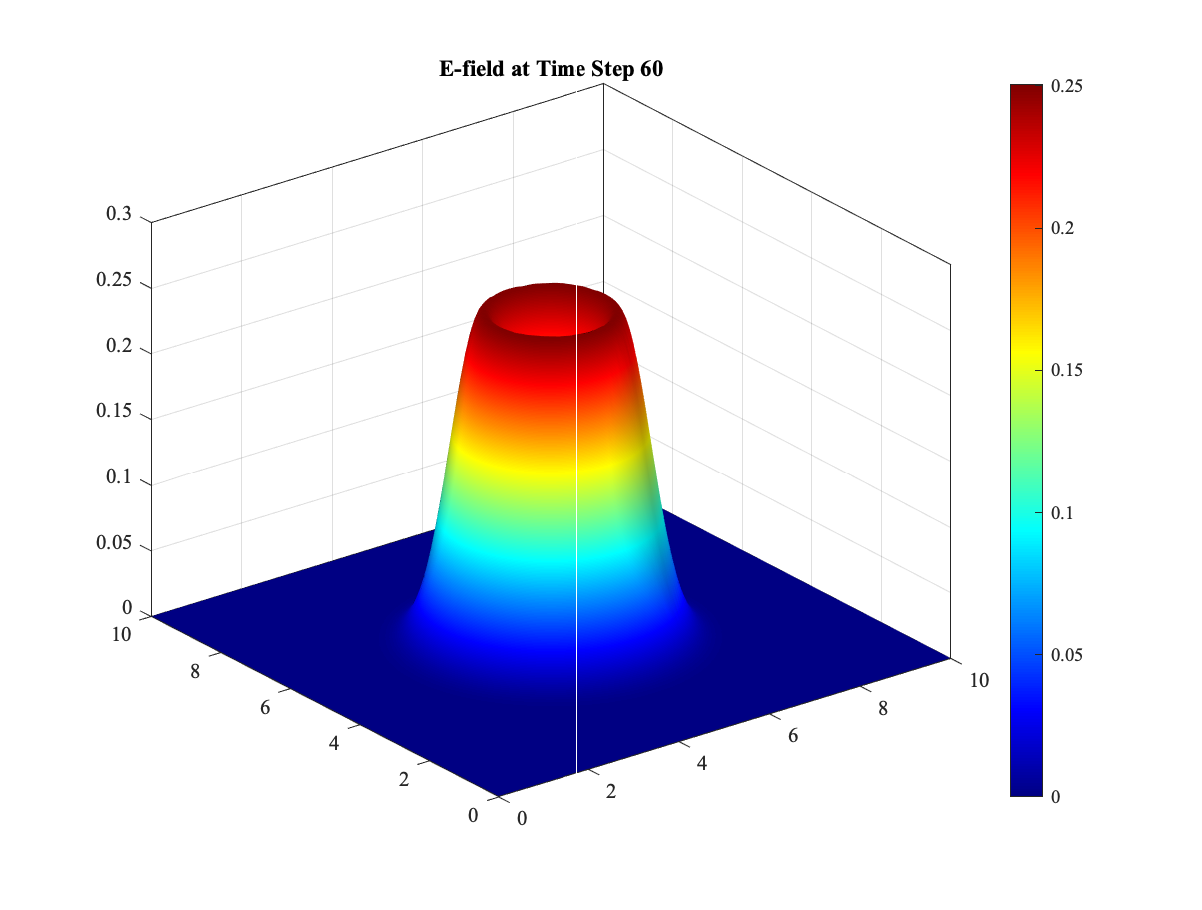
\includegraphics[width=2.5in]{Abbas_3_7_E_Field_60.eps}
  \label{fig:field_at_60}}
  \\
  \subfloat[80]{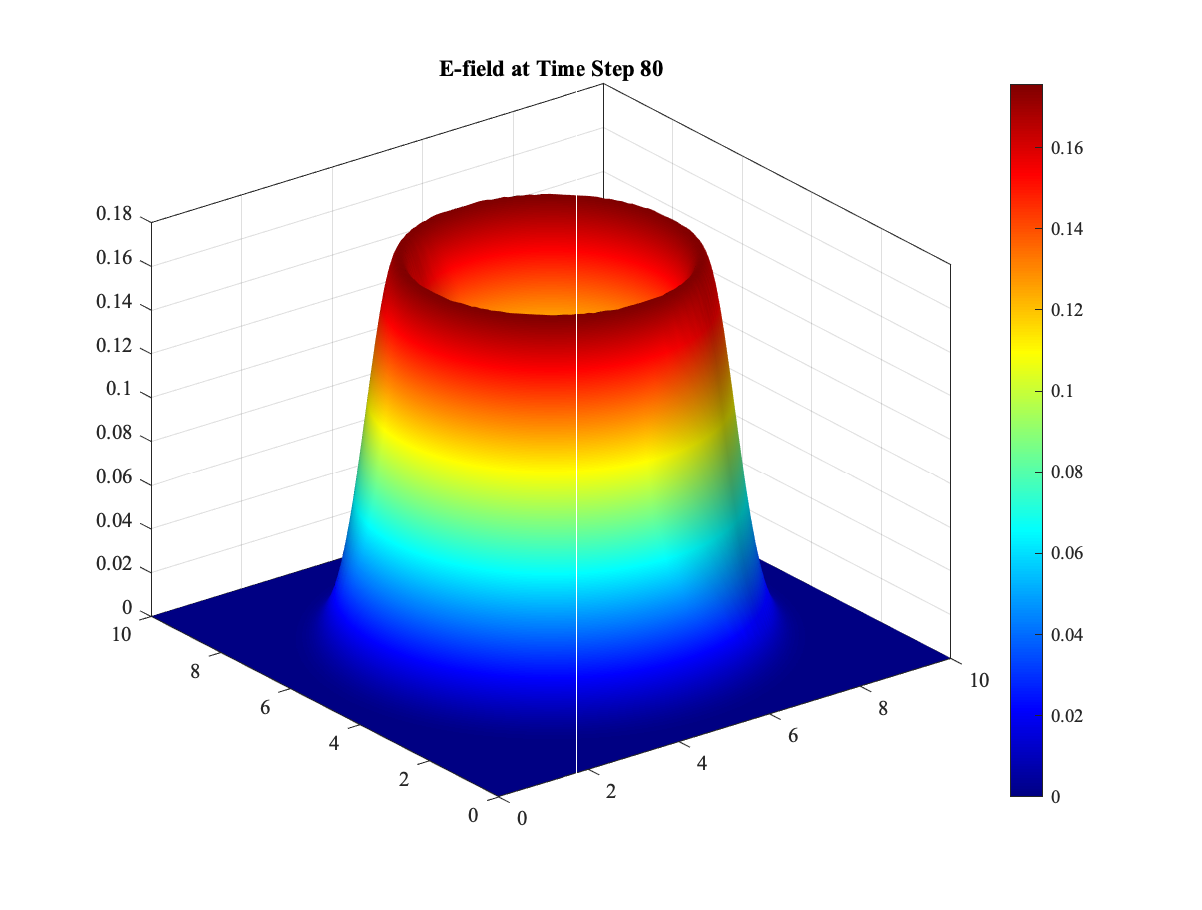
\includegraphics[width=2.5in]{Abbas_3_7_E_Field_80.eps}
  \label{fig:field_at_80}}
  \subfloat[160]{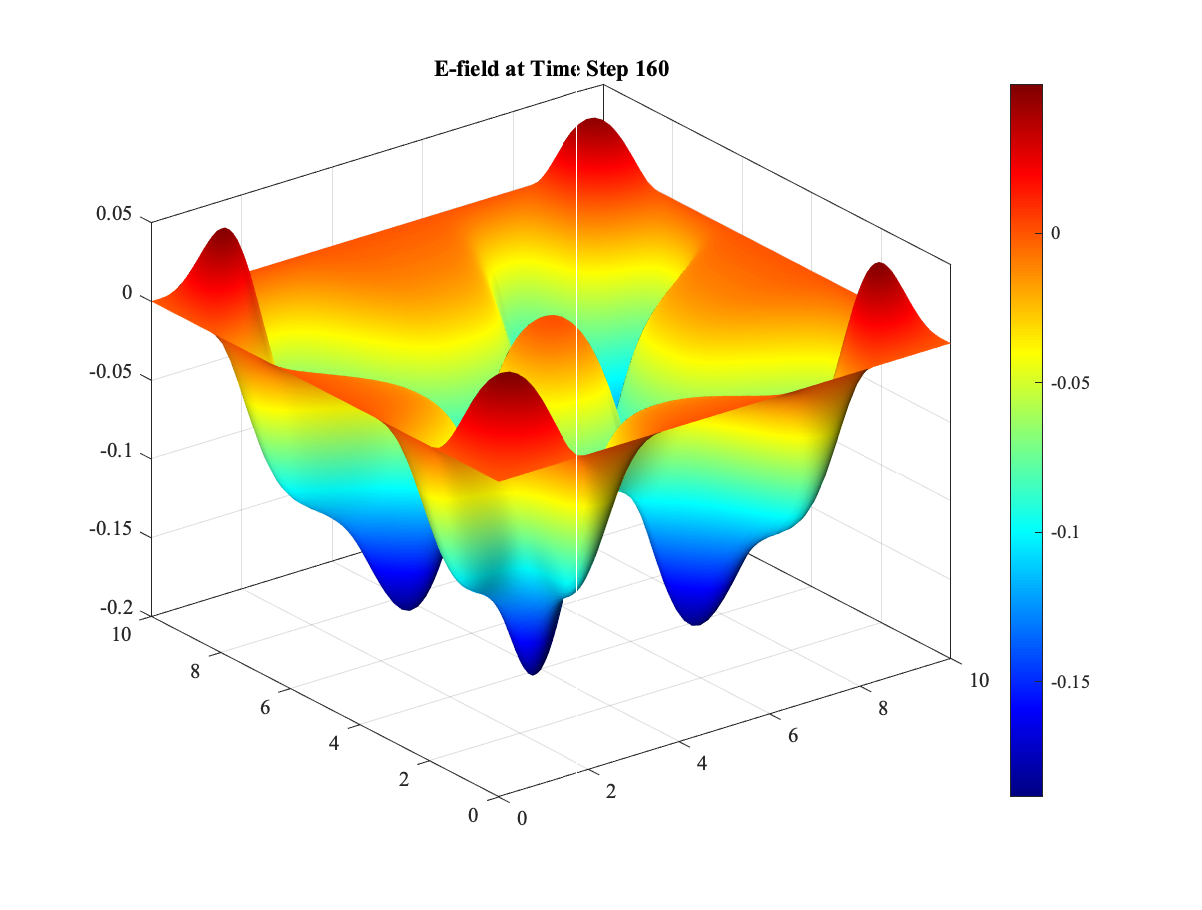
\includegraphics[width=2.5in]{Abbas_3_7_E_Field_160.eps}
  \label{fig:field_at_160}}
  \caption{The $E_z$ component visualised at different time intervals.}
  \label{fig:E_z fields}
\end{figure}

\subsection*{Exercise}

\begin{mdframed}[backgroundcolor=blue!20]
  Modify the above program to simulate the $TE$ mode. The expressions will be changed accordingly as provided in \eqref{eq:TE mode}.
\end{mdframed}


\section{Stability}

There has been extensive work done regarding the stability of the FDTD simulations. Stability ensures that any sources created don't shoot up in value as the simulation is progressed in time. As we saw in the lectures, the Courant number is a criterion for the stability of the FDTD simulation. It is different for 1-, 2-, and 3- dimensions. In order to find the stability conditions, the difference based Maxwell equations are treated as an eigenvalue problem and the eigenmodes determine the numerical stability. Essentially, we want to avoid the uncontrolled growth of all the possible spatial modes in the FDTD grid. As an example, a mode consisting of a sinusoidal function must have values in the limit $-1, \dots, 1$. Generally speaking, if we assume equal spatial spacing, ie, $\Delta_x = \Delta_y = \Delta_z = \Delta$, then a good rule of thumb for stability condition is:

\begin{align}
  \Delta_t \le \frac{\Delta}{2c}
\end{align}
where $c$ is the speed of light in the medium.

\subsection*{Exercise}

\begin{mdframed}[backgroundcolor=blue!20]

  Modify the stability condition in the Matlab routine (\texttt{Program 1.m}) to the following and plot the results at time instants 20, 40, 80, and 160.
  \scriptsize
  \begin{minted}{matlab}
% **************************
% **************************
dt = 1.3*ds/(c*sqrt(2)); % Stability Condition
% **************************
% **************************
  \end{minted}
\end{mdframed}
Also briefly explain what is happening in the simulation.

\section{Yee paper}

Let's try to replicate some of the results presented in Yee's seminal paper on FDTD \cite{kane_yee_numerical_1966}. The paper simulates a 2D $TM$ scattering problem, where there is a perfectly conducting square is placed at the centre. The square can be produced as below:

\begin{mdframed}[backgroundcolor=gray!20]
  \scriptsize
  \begin{minted}{matlab}
    %% Create Structure in the computational space
    % *************************
    % *************************
    function define_media(iflaga)
    
    global nx  ny mxst mxnd myst mynd;
    global mediaEz mediaHx mediaHy; %
    if (iflaga == 2)
        
        for  i = 1:nx
            for j = 1:ny
                if (i >= mxst && i <= mxnd)
                    if ( j >= myst && j <= mynd)
                        mediaEz(i,j) = 2;
                    end
                end
            end
        end
        
        for  i = 1:nx
            for j = 1:ny
                if (i >= mxst && i <= mxnd)
                    if ( j >= myst && j <= mynd-1)
                        mediaHx(i,j) = 2;
                    end
                end
            end
        end
        
        for  i = 1:nx
            for j = 1:ny
                if (i >= mxst && i <= mxnd-1)
                    if ( j >= myst && j <= mynd)
                        mediaHy(i,j) = 2;
                    end
                end
            end
        end
    end
    
    end
    
  \end{minted}
\end{mdframed}

Here the variable, \texttt{iflaga} either assumes the value 1 (free space) or 2 (PEC). The complete code can be found in the program \texttt{Program 2.m}. 


\subsection*{Exercise}

\begin{mdframed}[backgroundcolor=blue!20]

  Please run the program and produce the results for \texttt{n = 5} as shown in Figs 3 - 6 in \cite{kane_yee_numerical_1966}.
\end{mdframed}


\section{Boundary Conditions}

As we saw in class that we require FDTD to model \textit{open} regions where the spatial domain is unbounded. However, practically it is not possible as it requires an infinite amount of computer memory. Therefore, in order to limit the size of the simulation, we create a finite simulation domain with \textit{absorbing boundary conditions} (ABCs).  

A class of ABCs work on \textit{extrapolating} the field values at the boundary. One of the most famous ones is the Liao ABC \cite{liao_transmitting_1984} which works on updating the numerical fields in space and time using a Newton backward-difference polynomial.


The idea is that for any point on the grid bounday $x_{MAX}$, we need to calculate the updated field $u(x_{MAX}, t + \Delta_t)$ using the field values that we already have in the memory. As an example, the update field expressions for a 1D case can be written as:

\begin{align}
\Delta^1 E(x ,t) ={} & \Delta^1 E_1 = E_2 - E_1  = E(x,t) - E(x - \Delta_x, t - \Delta_t) \nonumber \\
\Delta^2 E_1 ={} & \Delta^1 E_1 - \Delta^1 E_2 \nonumber \\
={} & E(x,t) - \Delta^1 E(x - \Delta_x, t - \Delta_t) \nonumber \\
={} & E(x,t) - 2E(x - \Delta_x, t - \Delta_t) + E(x - 2\Delta_x, t - 2\Delta_t)
\end{align}

For the $N^{th}$ term, we get:

\begin{align}
  \Delta^N E(x ,t) ={} & \sum_{j = 1}^{N+1} C_{j-1}^{N} E\left[x - (j -1)\Delta_x, t - (j -1)\Delta_t\right] \nonumber \\
  \mathrm{where,} \, C_k^N ={} & \frac{\N\,!}{(N - k)\,! \, k\,!}
\end{align}

The \textit{extrapolation} can be understood from Fig. \ref{fig:backward_difference} where the point on the right is extrapolated from the neighbouring points, depending on the order of the Liao ABC.


\begin{figure}[t!]
  \centering
  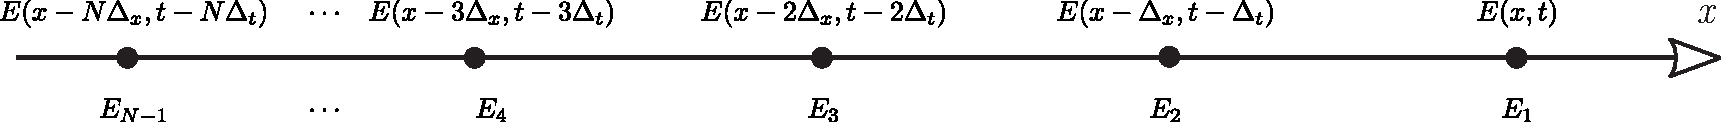
\includegraphics[width=0.9\textwidth]{backward difference.pdf}
  \caption{The backward difference used to compute the boundary points.}
  \label{fig:backward_difference}
\end{figure}

To implement the Liao ABCs in \texttt{MATLAB}, we first define the coefficients $C_k^N$ for a particular order. As an example, the $4-th$ order coefficients are:

\begin{mdframed}[backgroundcolor=gray!20]
  \scriptsize
  \begin{minted}{matlab}
    function define_Liao()

global c1 c2 c3 c4 c5 ; % Define material based coefficients
global ABC_order % Order of the Liao ABC 
switch ABC_order
  
        
    case 4 %% 4th order LIAO ABC Coefficients
        c1 = 4;
        c2 = 6;
        c3 = 4;
        c4 = 1;
        c5 = 0;
        
    otherwise
        disp('Error: Wrong Value')
end
end
  \end{minted}
\end{mdframed}

We then implement the Liao ABCs as:
\begin{mdframed}[backgroundcolor=gray!20]
  \scriptsize
  \begin{minted}{matlab}
    %% Implement LIAO ABC
    % *************************
    % *************************
    function Liao_ABC()
    
    global c1 c2 c3 c4 c5 ; % Define material based coefficients
    global Ez ; % E and H field components.
    global Ez1 Ez2 Ez3 Ez4 Ez5 % For Bubbling of E-fields in Liao ABC
    global nx  ny  
    global ABC_order
    % General BC for any order LIAO ABC
        for  j = 1:ny
        Ez(1,j) = c1*Ez1(2,j)-c2*Ez2(3,j)+c3*Ez3(4,j)...
             -c4*Ez4(5,j)+c5*Ez5(6,j);%%%left side
        end
        for j = 1:ny
        Ez(nx,j) = c1*Ez1(nx-1,j)-c2*Ez2(nx-2,j)+c3*Ez3(nx-3,j) ...
             -c4*Ez4(nx-4,j)+c5Ez5(nx-5,j);%%%right side
        end 
        for i = 2:nx-1
        Ez(i,1) = c1*Ez1(i,2)-c2*Ez2(i,3)+c3*Ez3(i,4) ...
            -c4*Ez4(i,5)+c5*Ez5(i,6);%%%bottom
        end
        for i = 2:nx-1
        Ez(i,ny) = c1*Ez1(i,ny-1)-c2*Ez2(i,ny-2)+c3*Ez3(i,ny-3) ...
             -c4*Ez4(i,ny-4)+c5*Ez5(i,ny-5);%%%top
        end
        
        switch ABC_order
            
            case 5
                Ez5 = Ez4;
                Ez4 = Ez3;
                Ez3 = Ez2;
                Ez2 = Ez1;
                Ez1 = Ez;
                
            case 4
                Ez4 = Ez3;
                Ez3 = Ez2;
                Ez2 = Ez1;
                Ez1 = Ez;
                
            case 3
                Ez3=Ez2;
                Ez2=Ez1;
                Ez1=Ez;
                
            otherwise
                disp('Error: Wrong Value')
        end
    end    
  \end{minted}
\end{mdframed}

In \texttt{Program 3.m}, the Liao ABCs are implemented for the same structure as in the Yee paper. 


\subsection*{Exercise}

\begin{mdframed}[backgroundcolor=blue!20]
  Plot the 1D electric fields at \texttt{n = 5} and try see how the  Figs 3 - 6 in \cite{kane_yee_numerical_1966} now look like.
\end{mdframed}


\subsection*{Home Exercise}

\begin{mdframed}[backgroundcolor=blue!20]
Create a sinusoidal source on the left boundary in a 2D $TM$ case and replace the PEC square in the Yee paper simulation with a dielectric square of $\E = 4$ of the same size.
\end{mdframed}

\section{Code Availability}

You can download the codes used in this manual from the \href{https://github.com/hasantahir/HFCS-Labs}{Github repository}.

\bibliography{references}
\bibliographystyle{ieeetran}
\end{document}
